% !TEX root = thesis.tex

\section{Results}
%In this section, we show the social prediction performance of the baseline results.
\subsection{Pre-processing Haggling Data}
Given the motion data of the Haggling games, we first annotate the start and end time of the game, where start time is decided when the social formation is built and the end time is defined when the social formation is broken. We crop out the motion dataset based on this start and end time, so that we ignore the time while subjects enter and exit the capture space. For each haggling game scene we also annotate the roles in the game, buyer, left-seller, and right-seller, where the left and right are determined in the buyer's view point. In our experiment we specify that the left seller is our target person and predict the social behavior of these subjects. Following the work of~\cite{holden2016deep}, we re-target the motion data to a standardized skeleton size to remove size variation from the body skeletons. We also synthesize footstep signals and decouple the body motion from global translation and orientation using the method of ~\cite{holden2016deep}. Finally we divide the dataset into 140 training sets and 40 test sets. However, since there exist sequences where the reconstruction errors are severe for some frames, we select only 79 training sets and 28 testing sets which are manually verified to be error free. Although our dataset captures face and body signals, we do not include these data in our current experiments. 


\subsection{Verification of Existing Theories (Proxemics)}
Our dataset has the measurement of fully voluntary motions of interacting people, and enables us to revisit the well-known proxemics theory~\cite{Hall66}. We first compute the average distance between a pair of subjects: (1) buyer and right sellers (B-RS), (2) buyer and left seller (B-LS), and (3) left seller and right seller (LS-RS). The results are shown in Table~\ref{table:proxemics_comp}. We found that the result approximately follows the social distance categories defined in the Hall's categorization~\cite{Hall66}. The distances among sellers are within the close phase of social distance ranges (from 120-210 $cm$) and the average distance among sellers and buyers are within the far phase of social distance (from 210 to 370 $cm$) in \cite{Hall66}. To analyze the shape of the social formation, we plot the average formation of games in a person-centric coordinate by a buyer. The results are shown in the Figure~\ref{fig:socialgeo_distribution}, showing that the formation is often similar to isosceles triangles with relatively far distances between a buyer and two sellers than the distance between sellers. 


\begin{table}[t]
	\centering
	\footnotesize
	\caption{Average distances (cm) between subjects. B, RS, and LS denote buyer, right seller, and left seller respectively.}
	\label{table:proxemics_comp}
	\begin{tabular}{l| l| l| l| l}
		\hline
		%Types & Avg. dist. (cm) & Std.(cm) & Min dist. (cm)  & Max dist. (cm)\\
		& Avg. dist. & Std. & Min & Max \\
		\hline
		B-RS & 148.11 & 27.26 & 99.03 & 265.52 \\
		\hline
		B-LS & 151.45 & 29.62 & 104.24  & 284.85 \\
		\hline
		LS-RS & 124.13 & 24.05  & 77.70  & 206.26 \\
		\hline
	\end{tabular}
\end{table}

\begin{figure}
	\centering       
	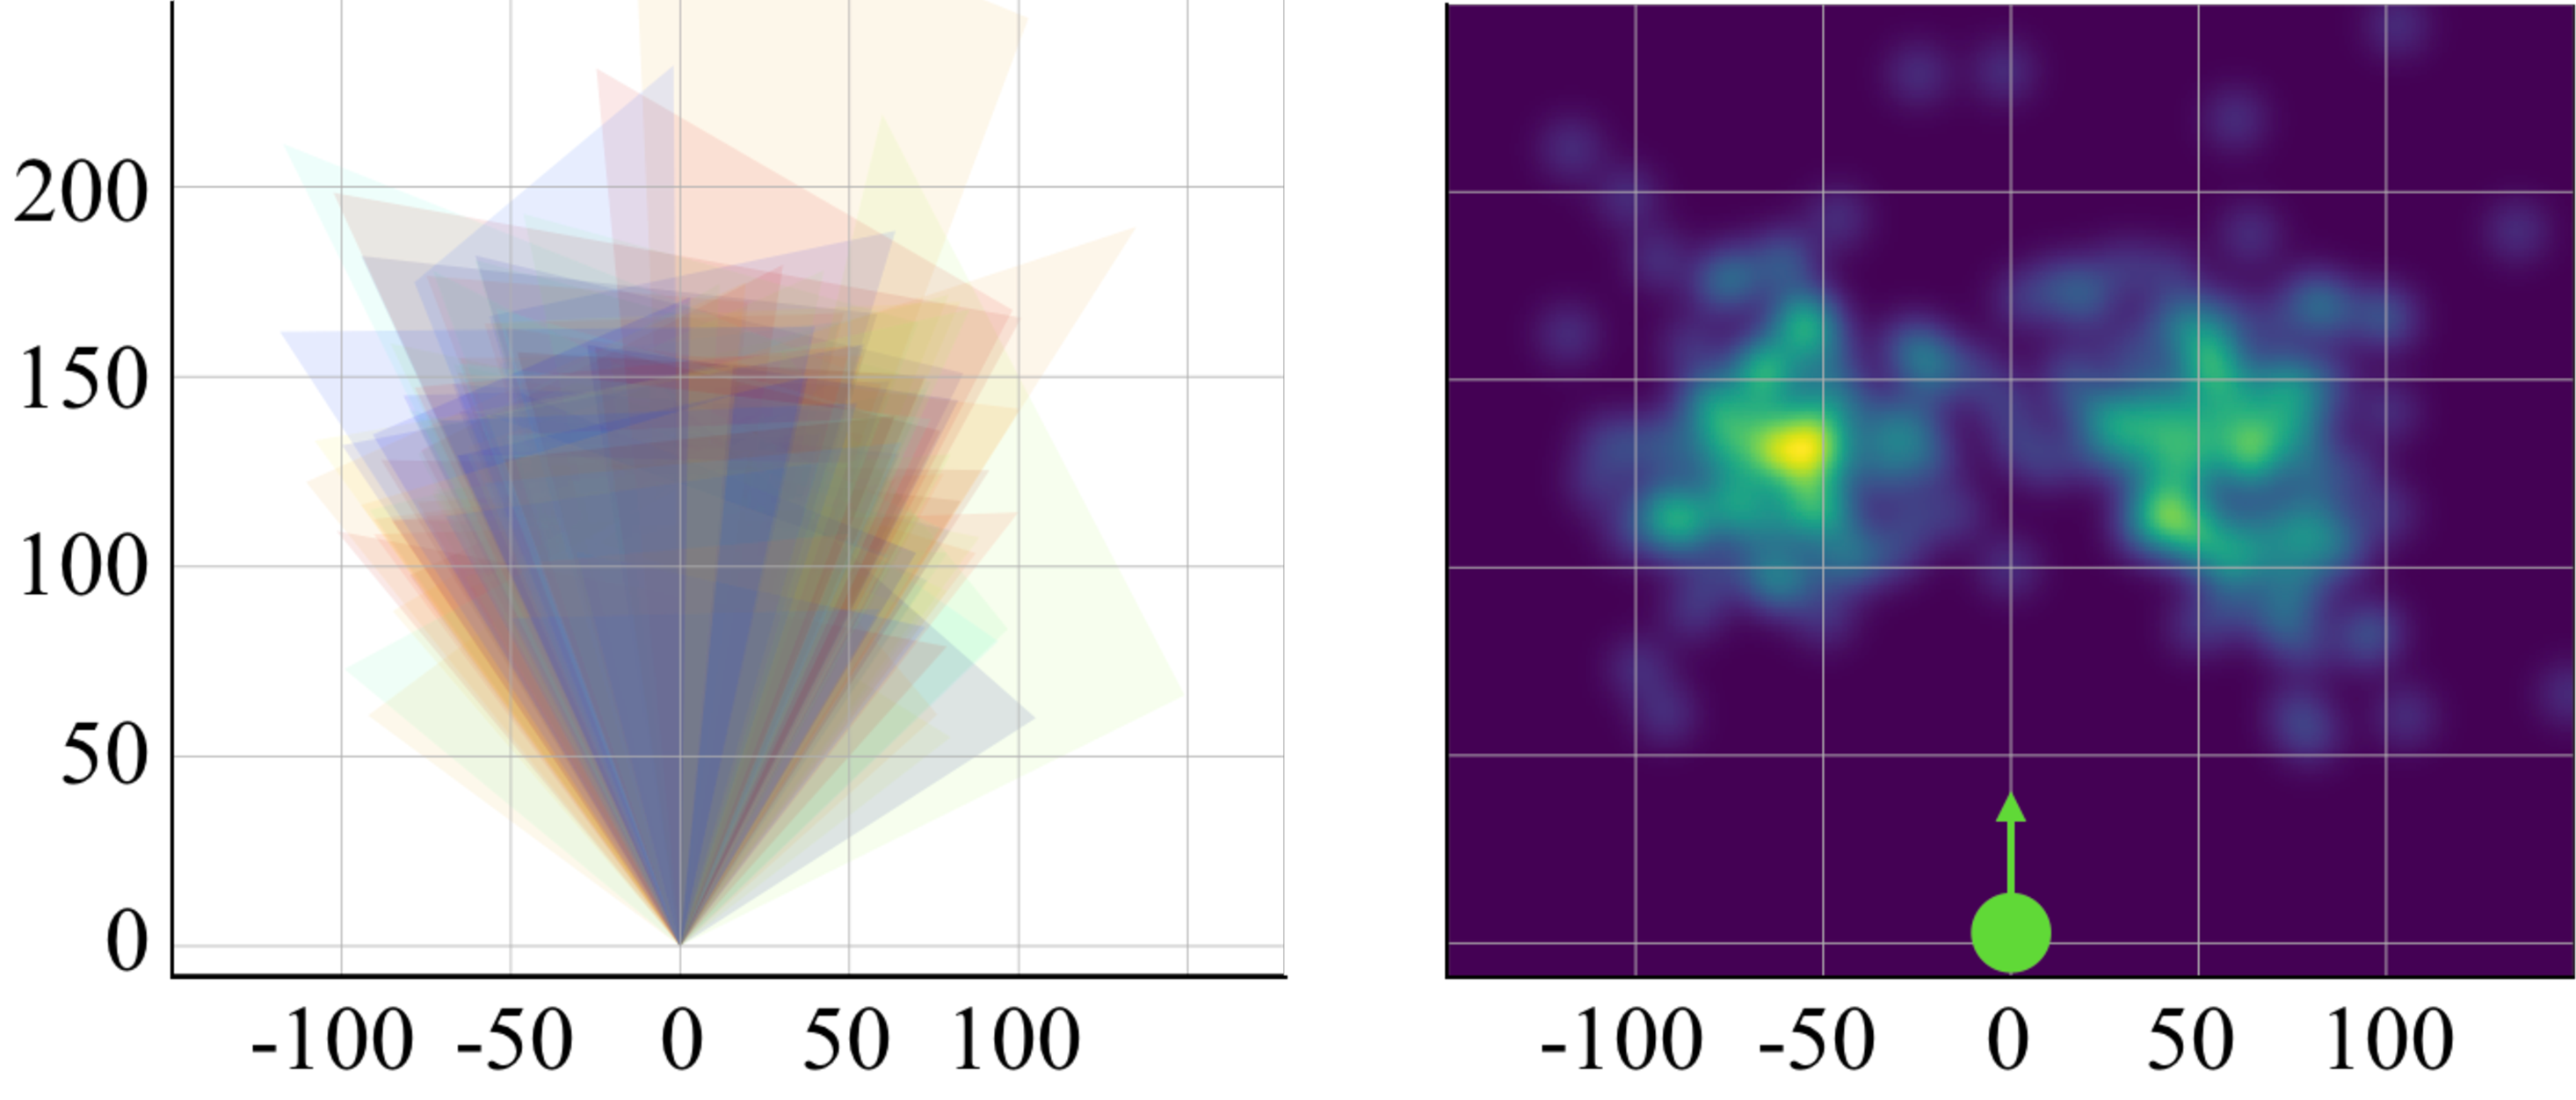
\includegraphics[ width=0.8\linewidth]{ssp_fig/haggling_proxemics_stat.pdf}
	% 	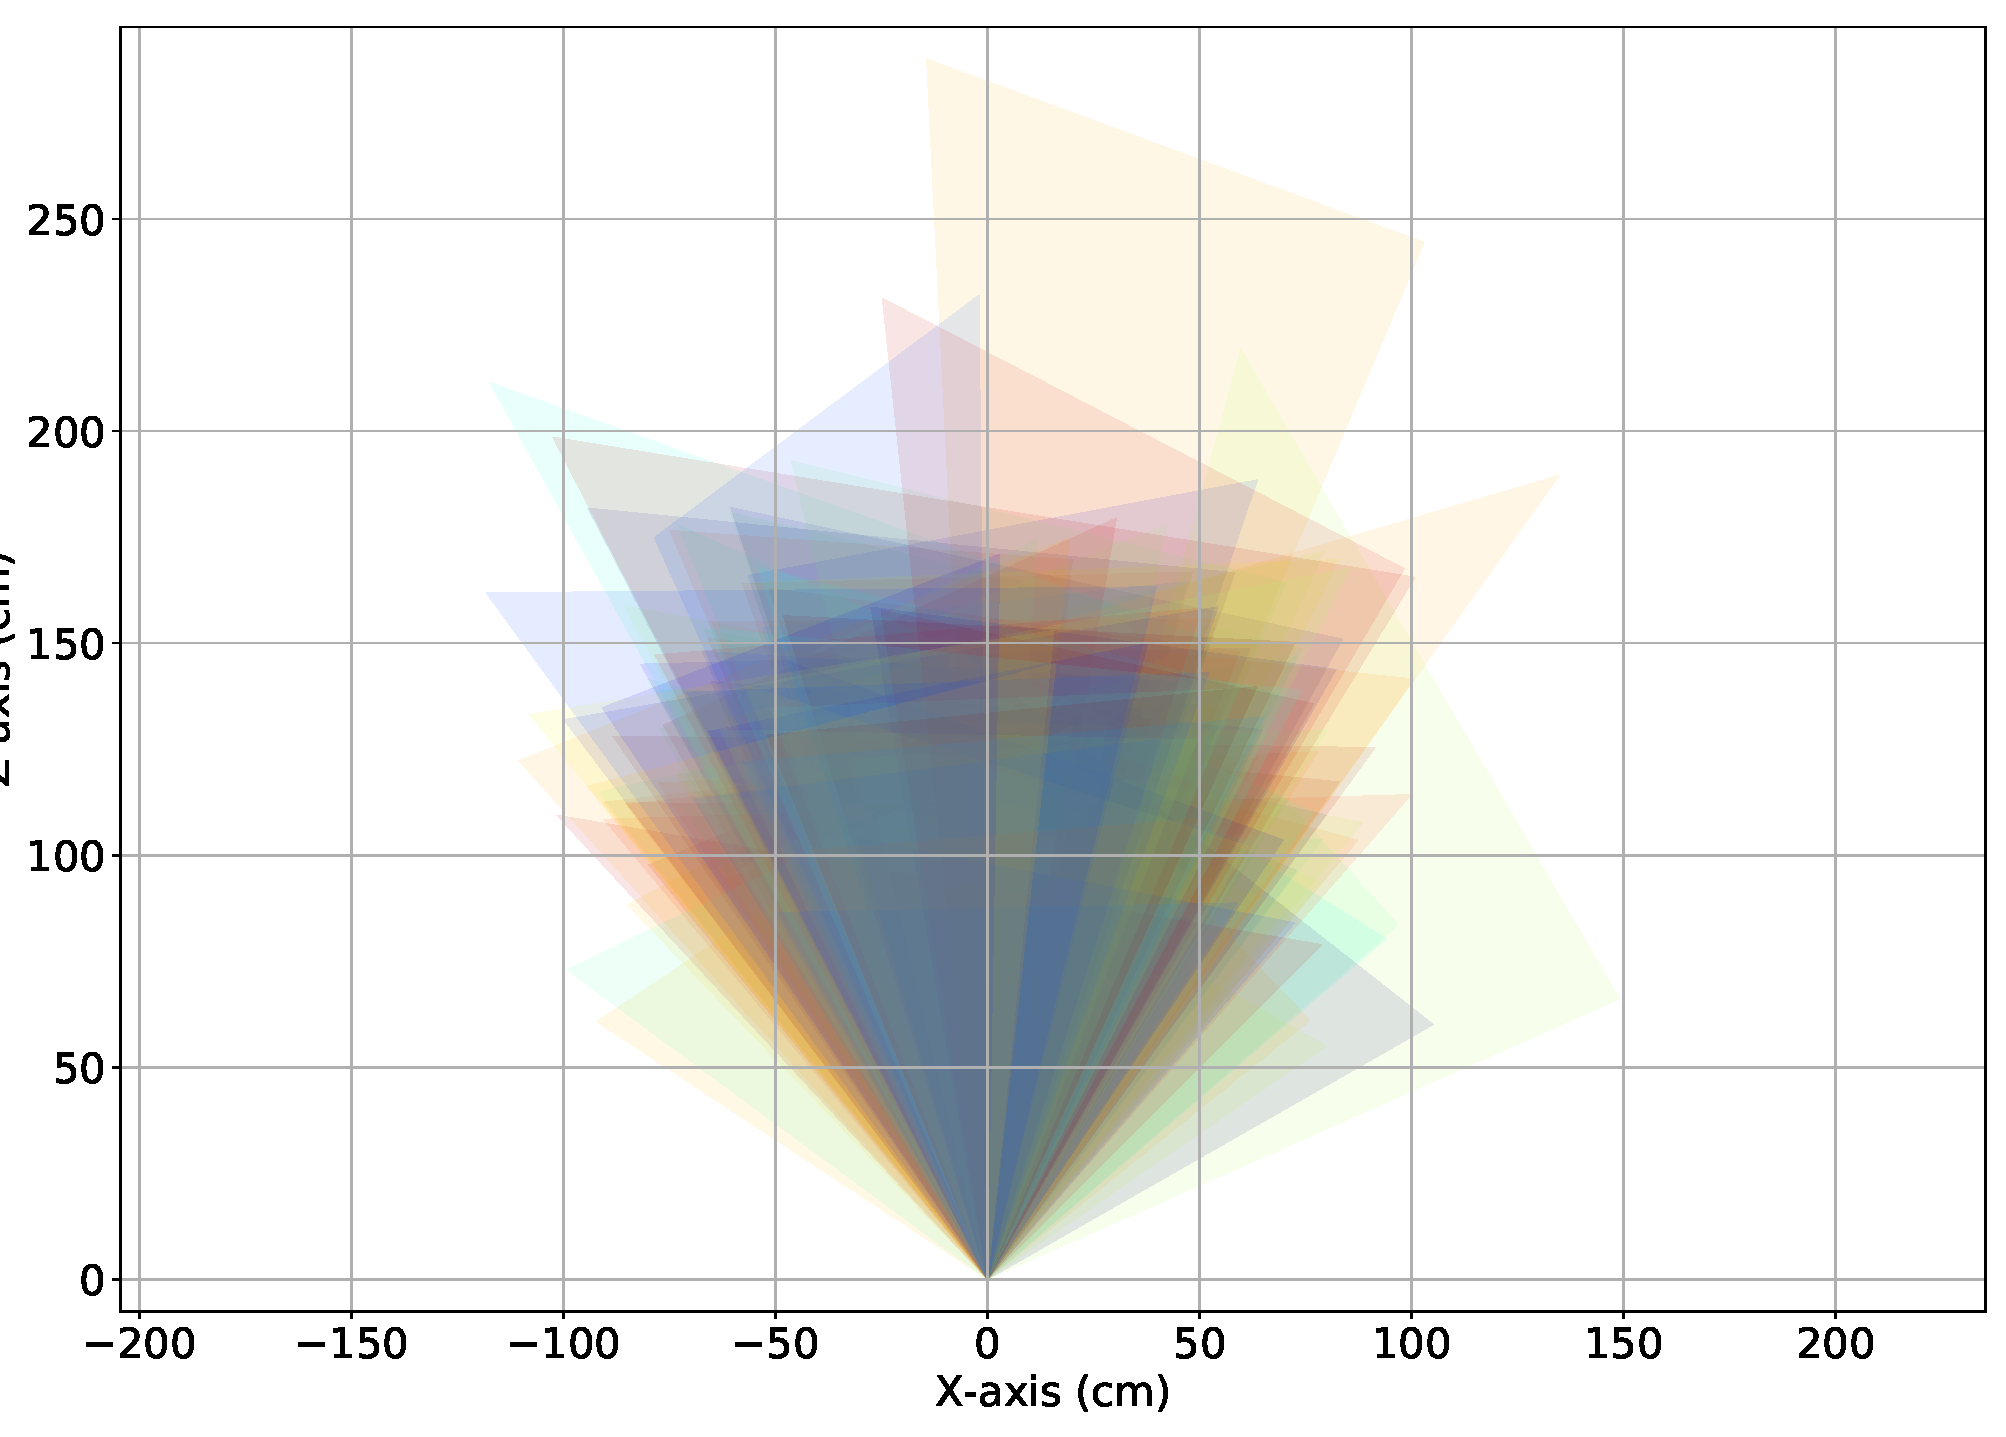
\includegraphics[trim=120 0 120 0,clip, width=0.45\linewidth]{plot/haggling_proxemics_polygon.pdf}
	% 	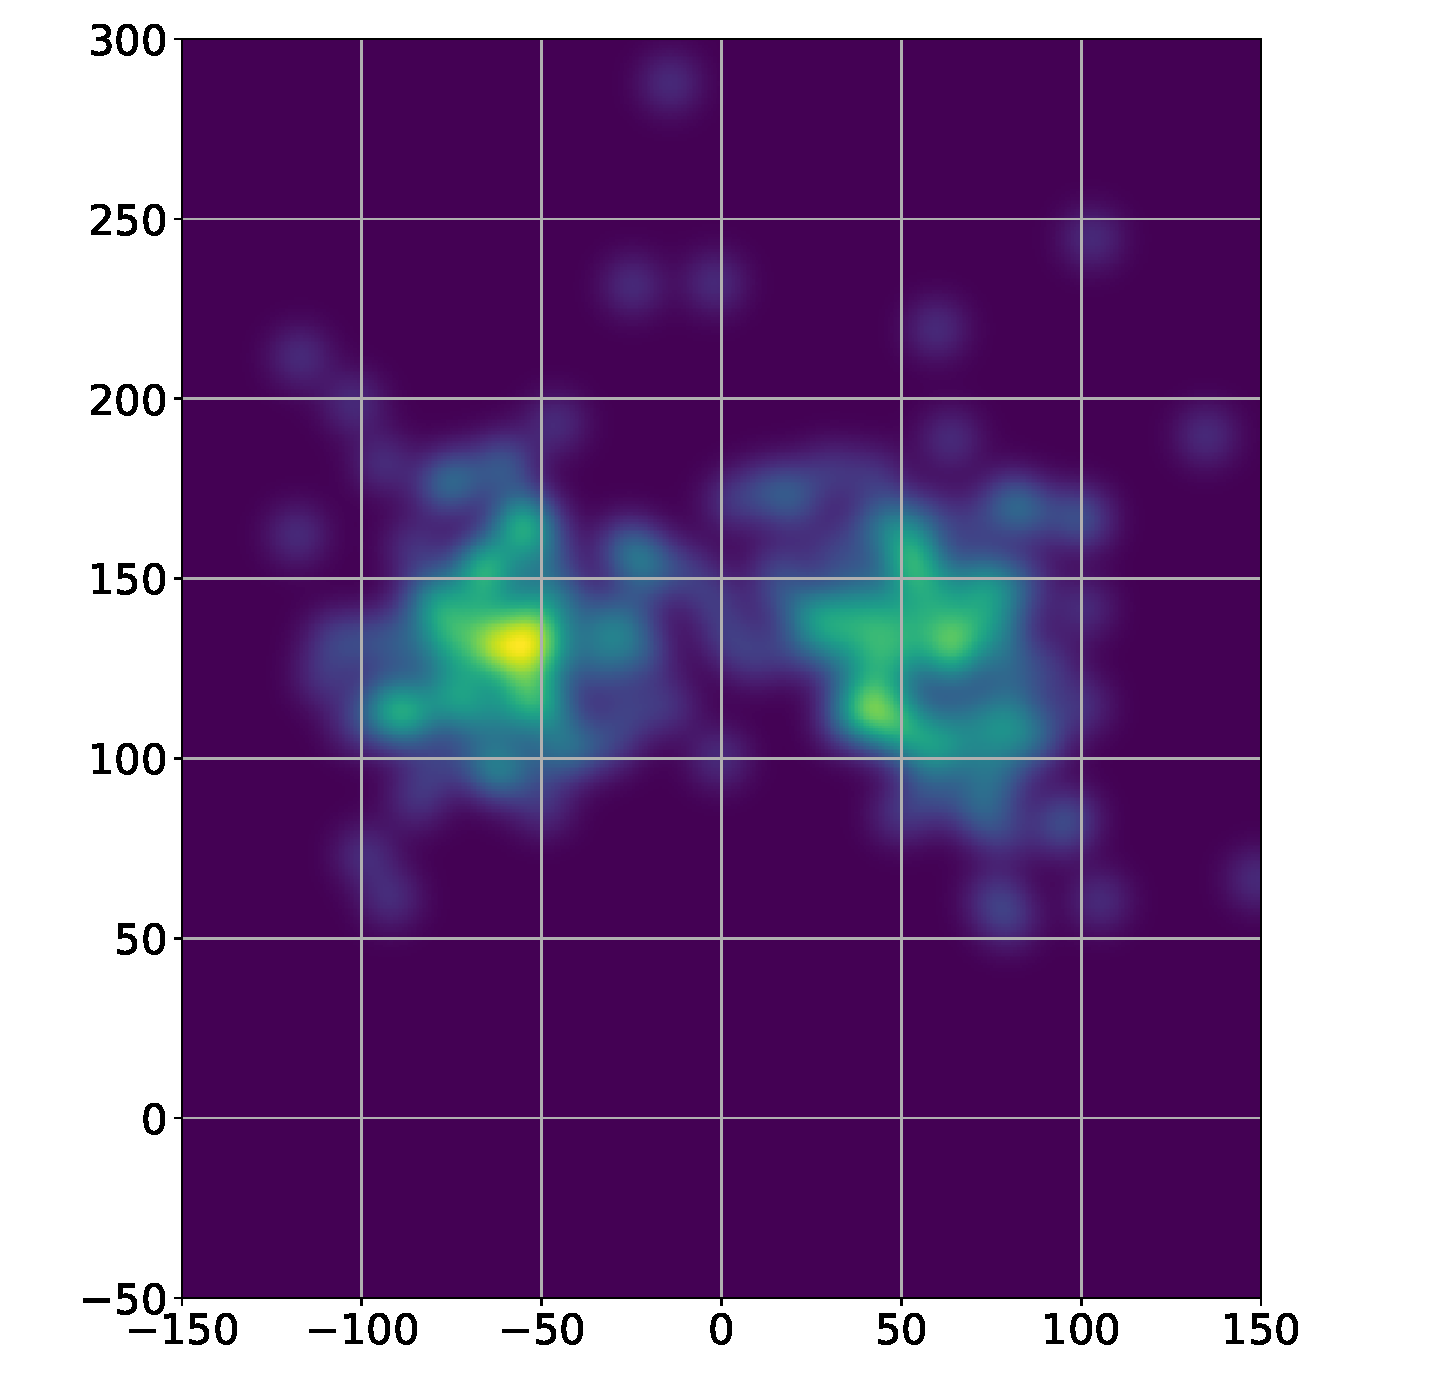
\includegraphics[width=0.45\linewidth]{plot/haggling_proxemics_heatmap.pdf} 
	%	\subfigure[TrajCompares]{\label{Fig:asso_traj}\includegraphics[width=0.5\textwidth]{img/trajCompare}}   
	\caption{Visualizing social formations in the haggling sequences as triangles (left) and a heat map (right). The formation is normalized w.r.t the buyer's location, and the green circle on the right shows the buyer location (origin) and orientation ($z$-axis).} 
	\label{fig:socialgeo_distribution}
\end{figure}

% \begin{figure}
% 	\centering       
% 	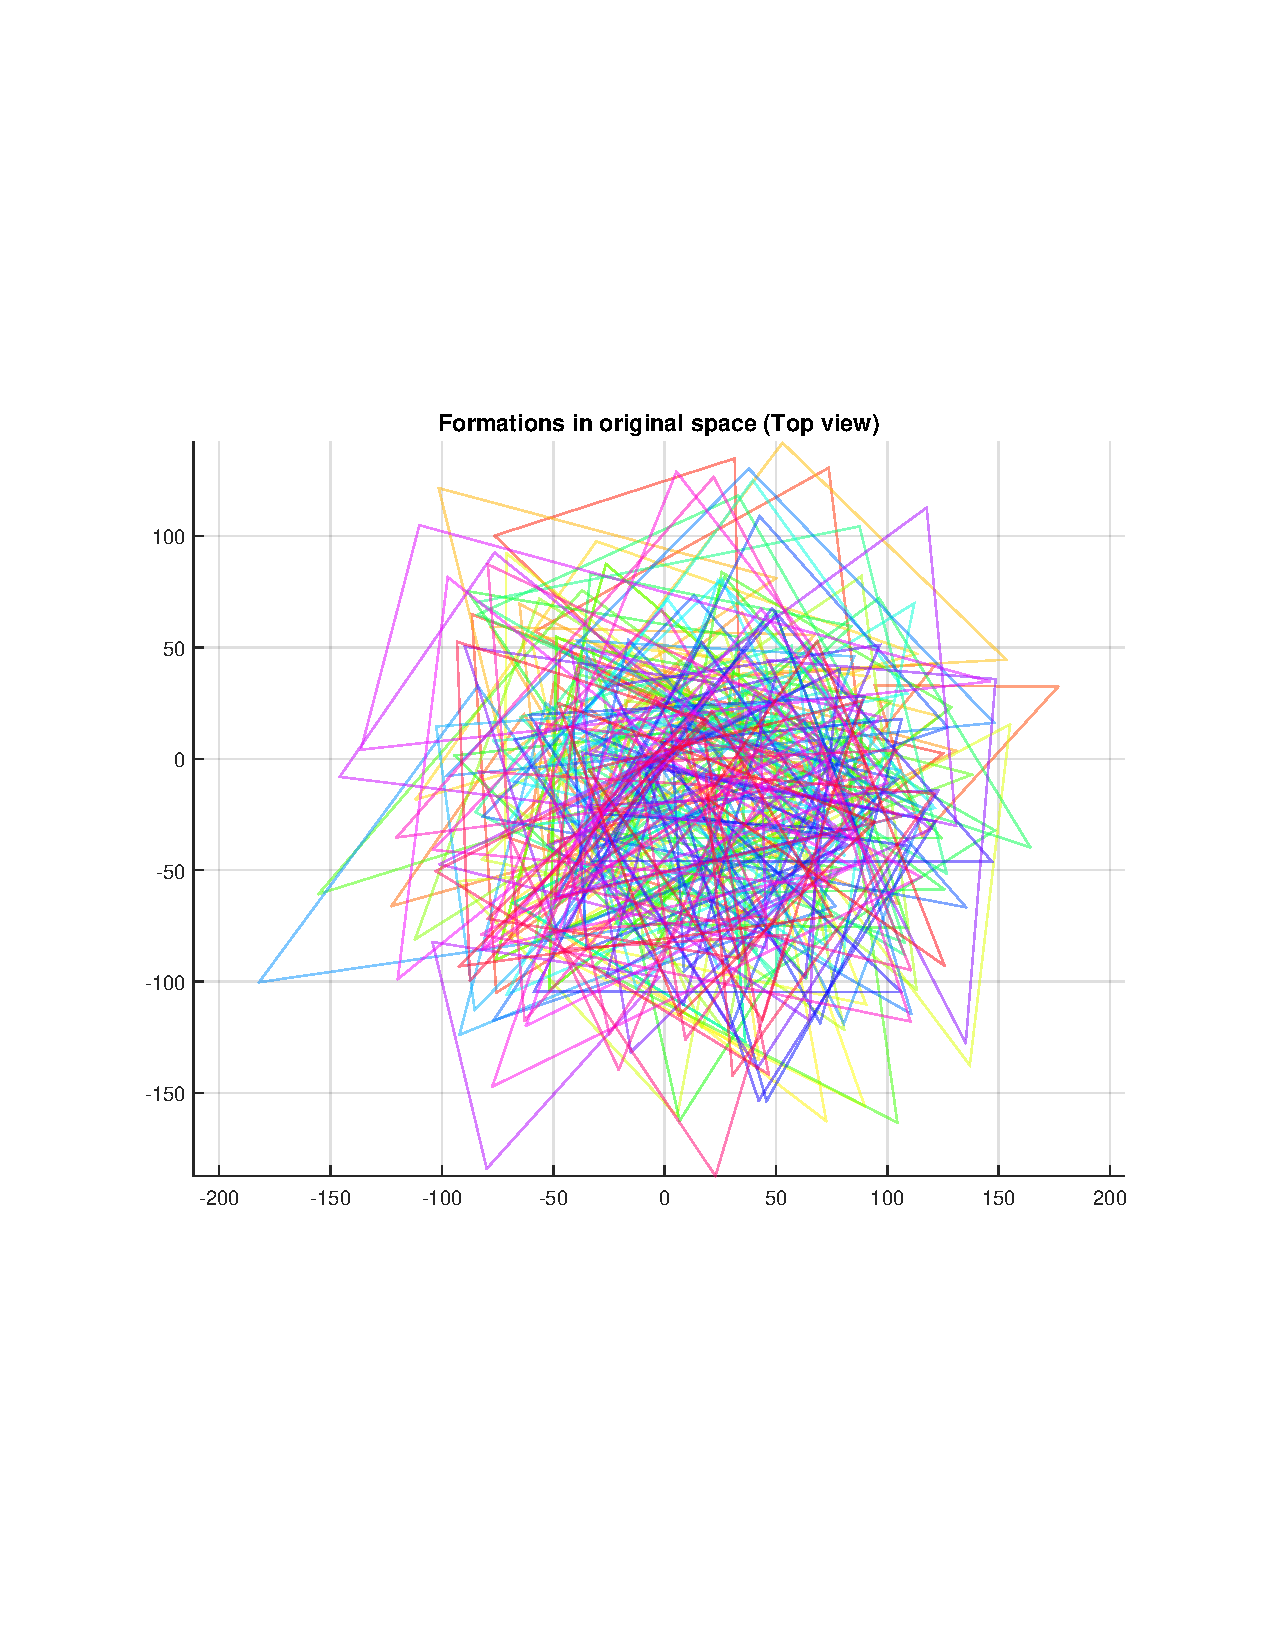
\includegraphics[trim=60 200 60 150,clip,width=0.32\linewidth]{fig/originalTri}
% 	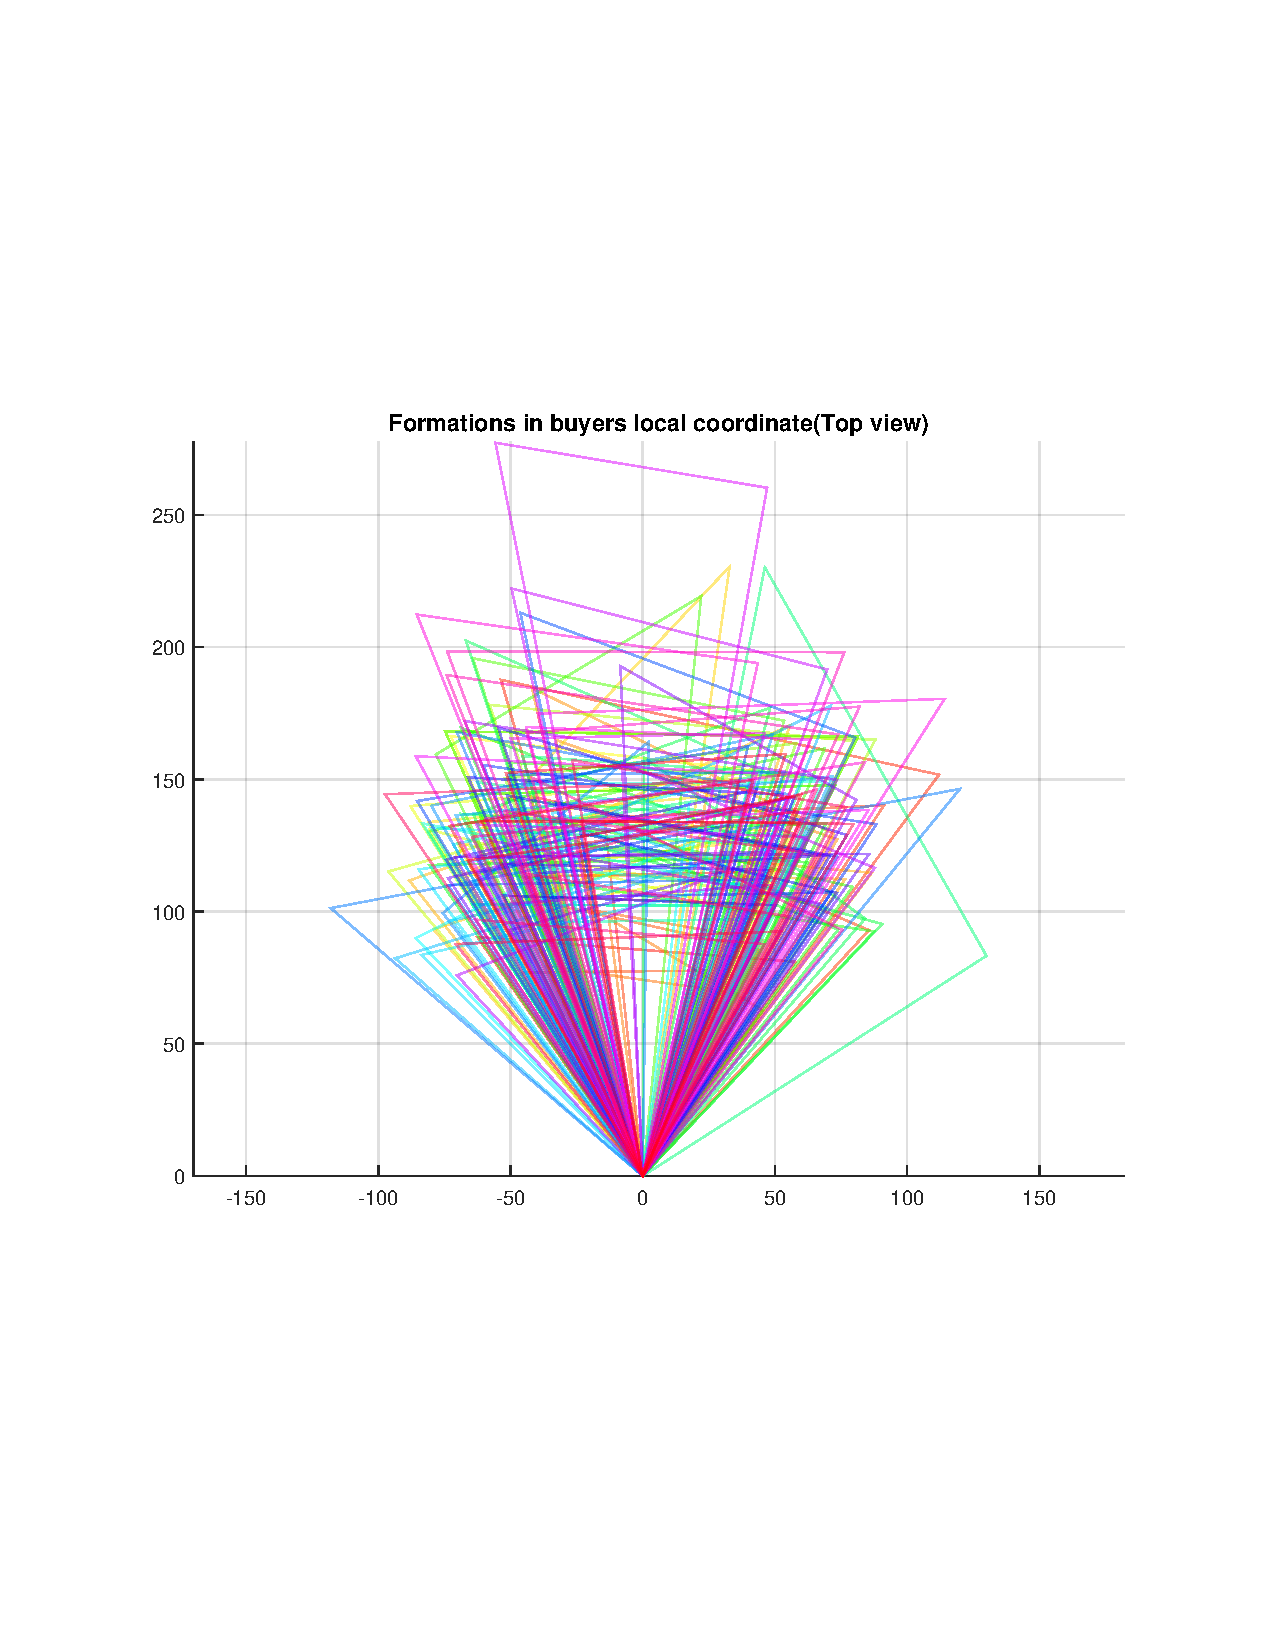
\includegraphics[trim=60 200 60 150,clip,width=0.32\linewidth]{fig/buyersTri} 
% 	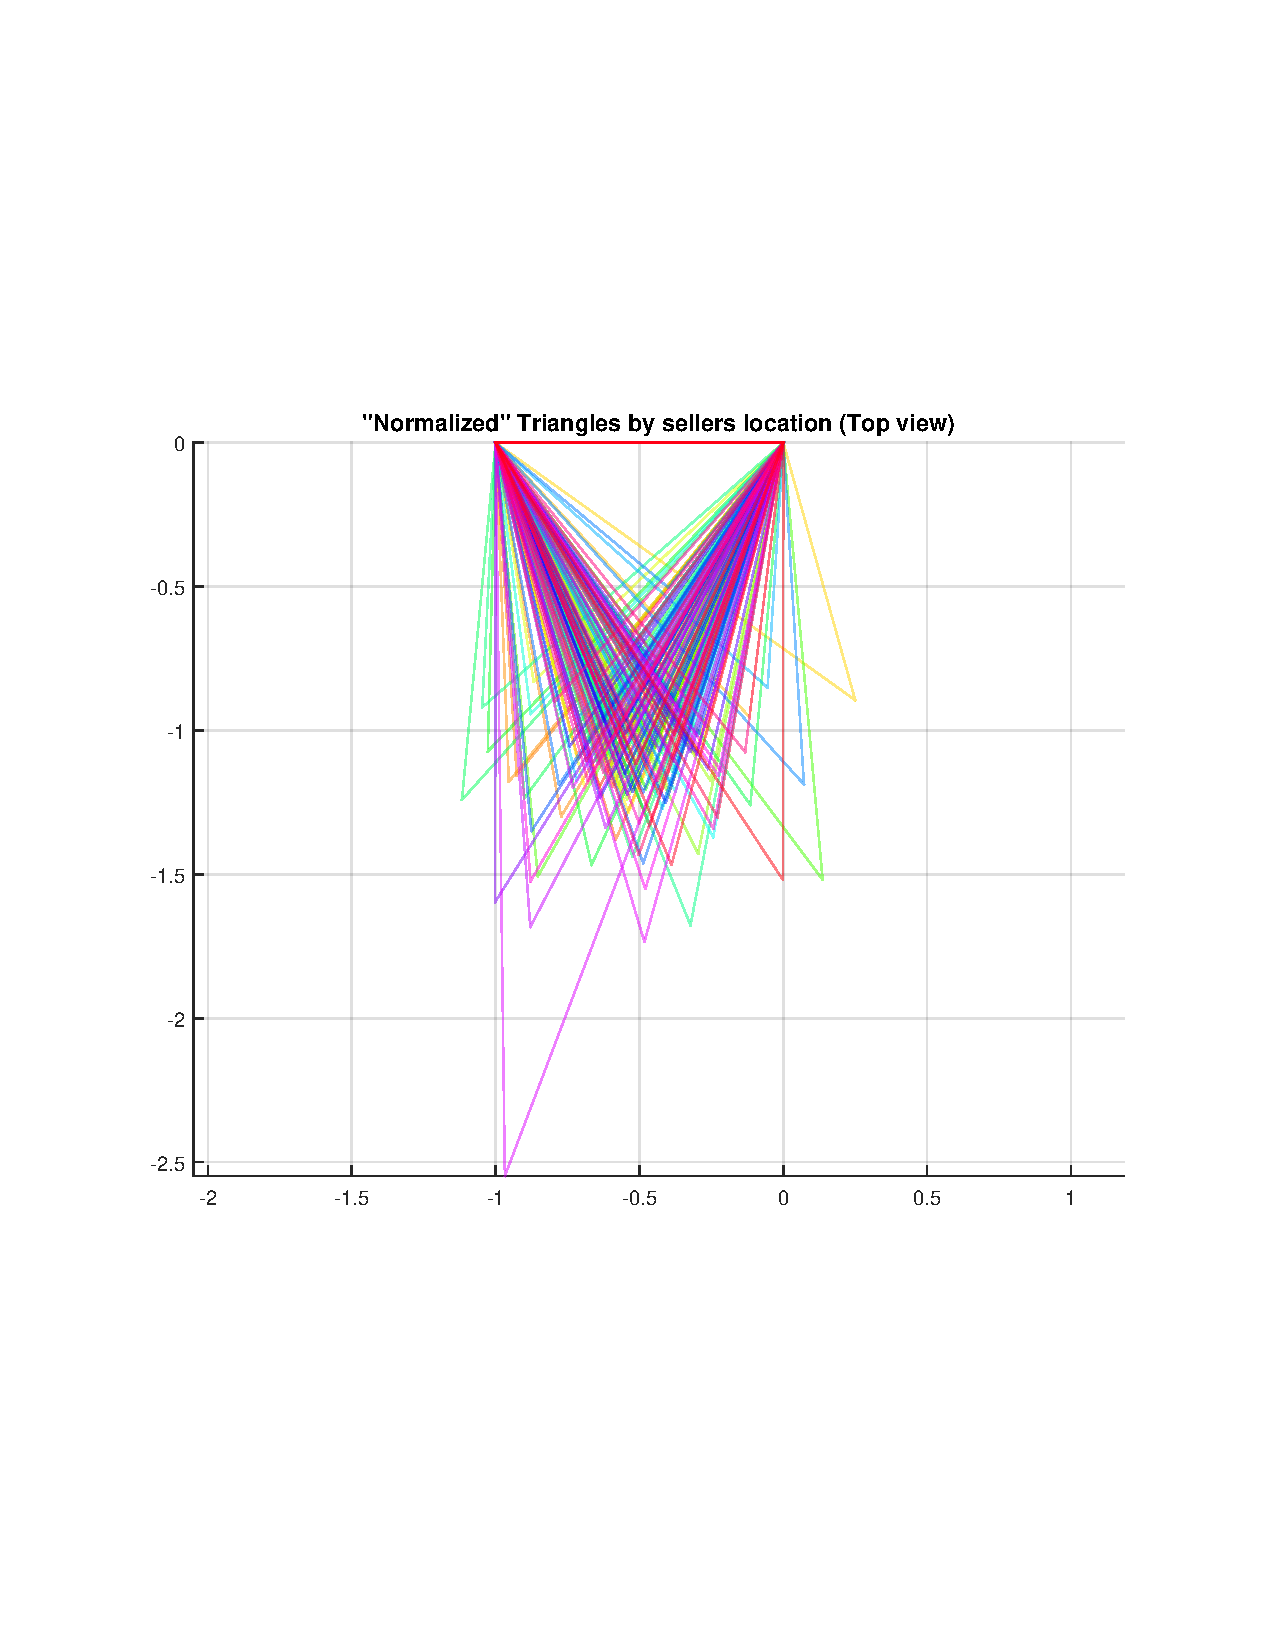
\includegraphics[trim=60 200 60 150,clip,width=0.32\linewidth]{fig/normTri} 
% 	%	\subfigure[TrajCompares]{\label{Fig:asso_traj}\includegraphics[width=0.5\textwidth]{img/trajCompare}}   
% 	\caption{Social formations in three different representations. (a) Global coordinate; (2) Person-centric coordinate defined by buyers; (3) Normalized-by-a-pair coordinate system define by two sellers} 
% 	\label{fig:socialgeo_distribution}
% \end{figure}

\subsection{Speaking Classification}
We compare the binary speaking classification performance in Table ~\ref{table:speaking_class}. The task is to classify the speaking status of the target person, and we use three different body motion sources: (1) the target person's own body motion, (2) the other seller's body motion, (3) a random person's body motion. As shown in the results, the own body motion has the strongest correlation, but the other seller's body motion is also very predictive, showing that there exists a clear social link during their interaction. As expected, the classification performance using a random person's motion as input shows about the chance level (50\%). For the experiment (3), we use the same network trained for (2), but use the body motion from a subject in some other arbitrary sequence (excluding our current target sequence) as input. Presumably, the classification method using the other person's body signals learns the ``turn-taking" property in the social interaction, and predicts that the target person is speaking if little motion is observed from the other sellers (who would be listening). %This kind of study is important to make machines better understand human social behaviors, and can be facilitated from the data where natural social interactions are captured.  %This kin %shows an interesting insight that the body motions % the strong correlation of social signals can be used as a prior for predicting human behaviors. 
\begin{table}[t]
	\centering
	\footnotesize
	\caption{Speaking Classification Accuracy using different source of body motion signals as input}
	\label{table:speaking_class}
	\begin{tabular}{l| l| l| l}
		\hline
		%Types & Avg. dist. (cm) & Std.(cm) & Min dist. (cm)  & Max dist. (cm)\\
		Input Signal & Own body & Other seller & Random person\\
		\hline
		%Accuracy & 80.34\% & 73.44\% & 53.39\%\\
		%Accuracy & 76.16\% & 70.33\% & 51.05\%\\       %submitted
		Accuracy & 80.70\% & 75.30\% & 51.05\%\\       %new
		\hline
	\end{tabular}
\end{table}


\subsection{Social Formation Prediction}
We predict the formation of social interaction by predicting the location and orientations of the target person, ``left seller". Fig.~\ref{fig:predForm_errors} and Table~\ref{table:predForm_errors} show the results. Our method shows a 25 cm error in the prediction, which is better than a baseline. As the baseline, we predict the location of the target seller to mirror that of the other seller w.r.t the buyer's body orientation, and estimate body orientation as the average between the two input subjects. The face orientation is chosen to always face the buyer (denoted as ``Mirroring" in Table~\ref{table:predForm_errors}). We also perform an ablation study to see what information is important to get better accuracy. To do this, we change the channel of the input, as in Table~\ref{table:predForm_errors}. To do this, we use the same network  but set unused input channels to their mean values in the training set. This experiment demonstrates that social formation estimation can take advantages from the body and face orientation signals. Intuitively, we can imagine that the target person's location can be estimated by triangulating the face normal direction of the other two subjects. To compute errors of orientations, we compute the 2D distance between the unit vectors representing the orientation estimation and the ground truth normal directions of face or body. In Fig.~\ref{fig:predForm_errors}, the average position errors of each sequences are shown. 

\begin{figure}
	\centering
	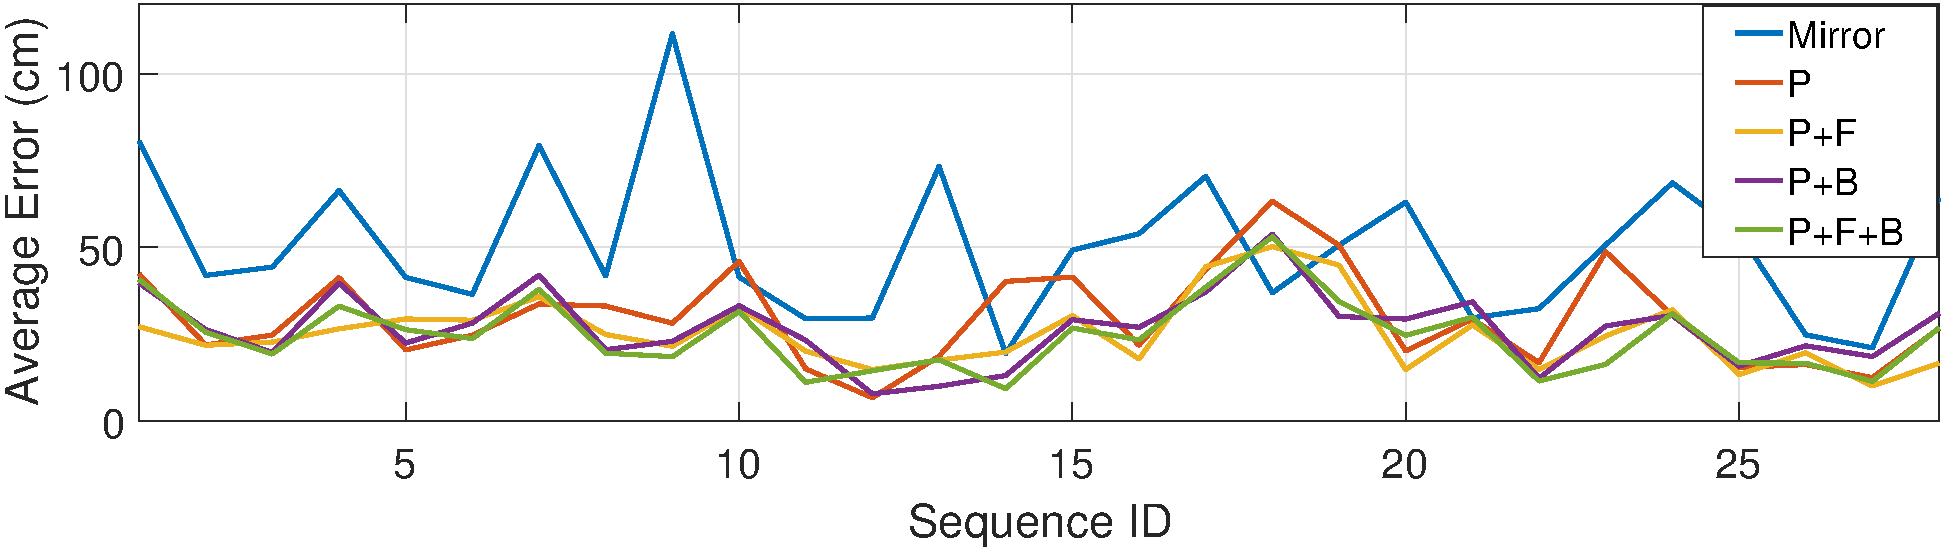
\includegraphics[width=\linewidth]{ssp_fig/cvpr19_predForm}\\
	\includegraphics[width=\linewidth]{ssp_fig/cvpr19_predBody}
	\caption{Average error of social formation prediction (top) and body gesture prediction (bottom). $y$-axis for the position errors in centimeters, and $x$-axis is sequence IDs.} %``Mirror" represents the baseline method, and P, F, and B denote Position, Face orientation, and Body orientation, as the input for the prediction.} 
	\label{fig:predForm_errors}
\end{figure}


\begin{table}[t]
	\centering
%	\small
	%\caption{Social Formation Prediction Errors (cm) }
	\begin{tabular}{l| l| l| l}
		\hline
		%Types & Avg. dist. (cm) & Std.(cm) & Min dist. (cm)  & Max dist. (cm)\\
		Types & Pos. & Body Ori & Face Ori\\
		\hline
		Mirroring &  50.03 (20.84) & 0.40 (0.17) & 0.52 (0.14) \\
		\hline
		PosOnly & 29.83 (13.38) & 0.26 (0.12) & 0.33 (0.13) \\
		\hline
		Pos+face & 25.23 (9.74) & 0.23 (0.09) & 0.30 (0.12) \\
		\hline
		Pos+body & 26.57 (10.24) & 0.22 (0.08) & 0.30 (0.10) \\
		\hline
		Pose+face+body & \underline {\textbf{24.59}} (10.23) &  \underline {\textbf{0.21}} (0.06) &  \underline {\textbf{0.29}} (0.09) \\
		\hline
	\end{tabular}
	\label{table:predForm_errors}
	\caption{Social Formation Prediction Errors (cm). Average position error between our estimation and ground-truth are reported in centimeters. The body orientation and face orientation are computed between the distance of estimated facial/body normal direction and GTs.}
\end{table}

% %Body only
% total_avg_posErr: 29.8286890398, std 13.3812589645
% total_avg_bodyOriErr: 0.263378293988, std 0.124290071428
% total_avg_faceOriErr: 0.327747834313, std 0.129691809416

% %Body + face
% total_avg_posErr: 25.2330815723, std 9.74251270294
% total_avg_bodyOriErr: 0.228412316901, std 0.0890485420823
% total_avg_faceOriErr: 0.303724261948, std 0.116639345884

% %Body + bodyOri
% total_avg_posErr: 26.57, std 10.24
% total_avg_bodyOriErr: 0.22, std 0.08
% total_avg_faceOriErr: 0.30, std 0.10

%While lower error may mean a better result, we may still see whether the prediction behave as human. 
% {\color{red} What happen when the turns are changing }

% {\color{red} Failure cases?}

% Position only, and orientation. 

% W/Wo speaking

% W/Wo body signal

% PCK curves

% Baseline: Trianglular estimation
% Orientation: See always the buyer.

% \begin{figure}
% 	\centering
% 	\includegraphics[width=\linewidth]{plot/cvpr19_predBody}
% 	\caption{Average error of body prediction. $y$-axis for the errors in centimeter, and $x$-axis for the sequences.} 
% 	\label{fig:predBody_errors}
% \end{figure}

\begin{figure*}
	\centering       
	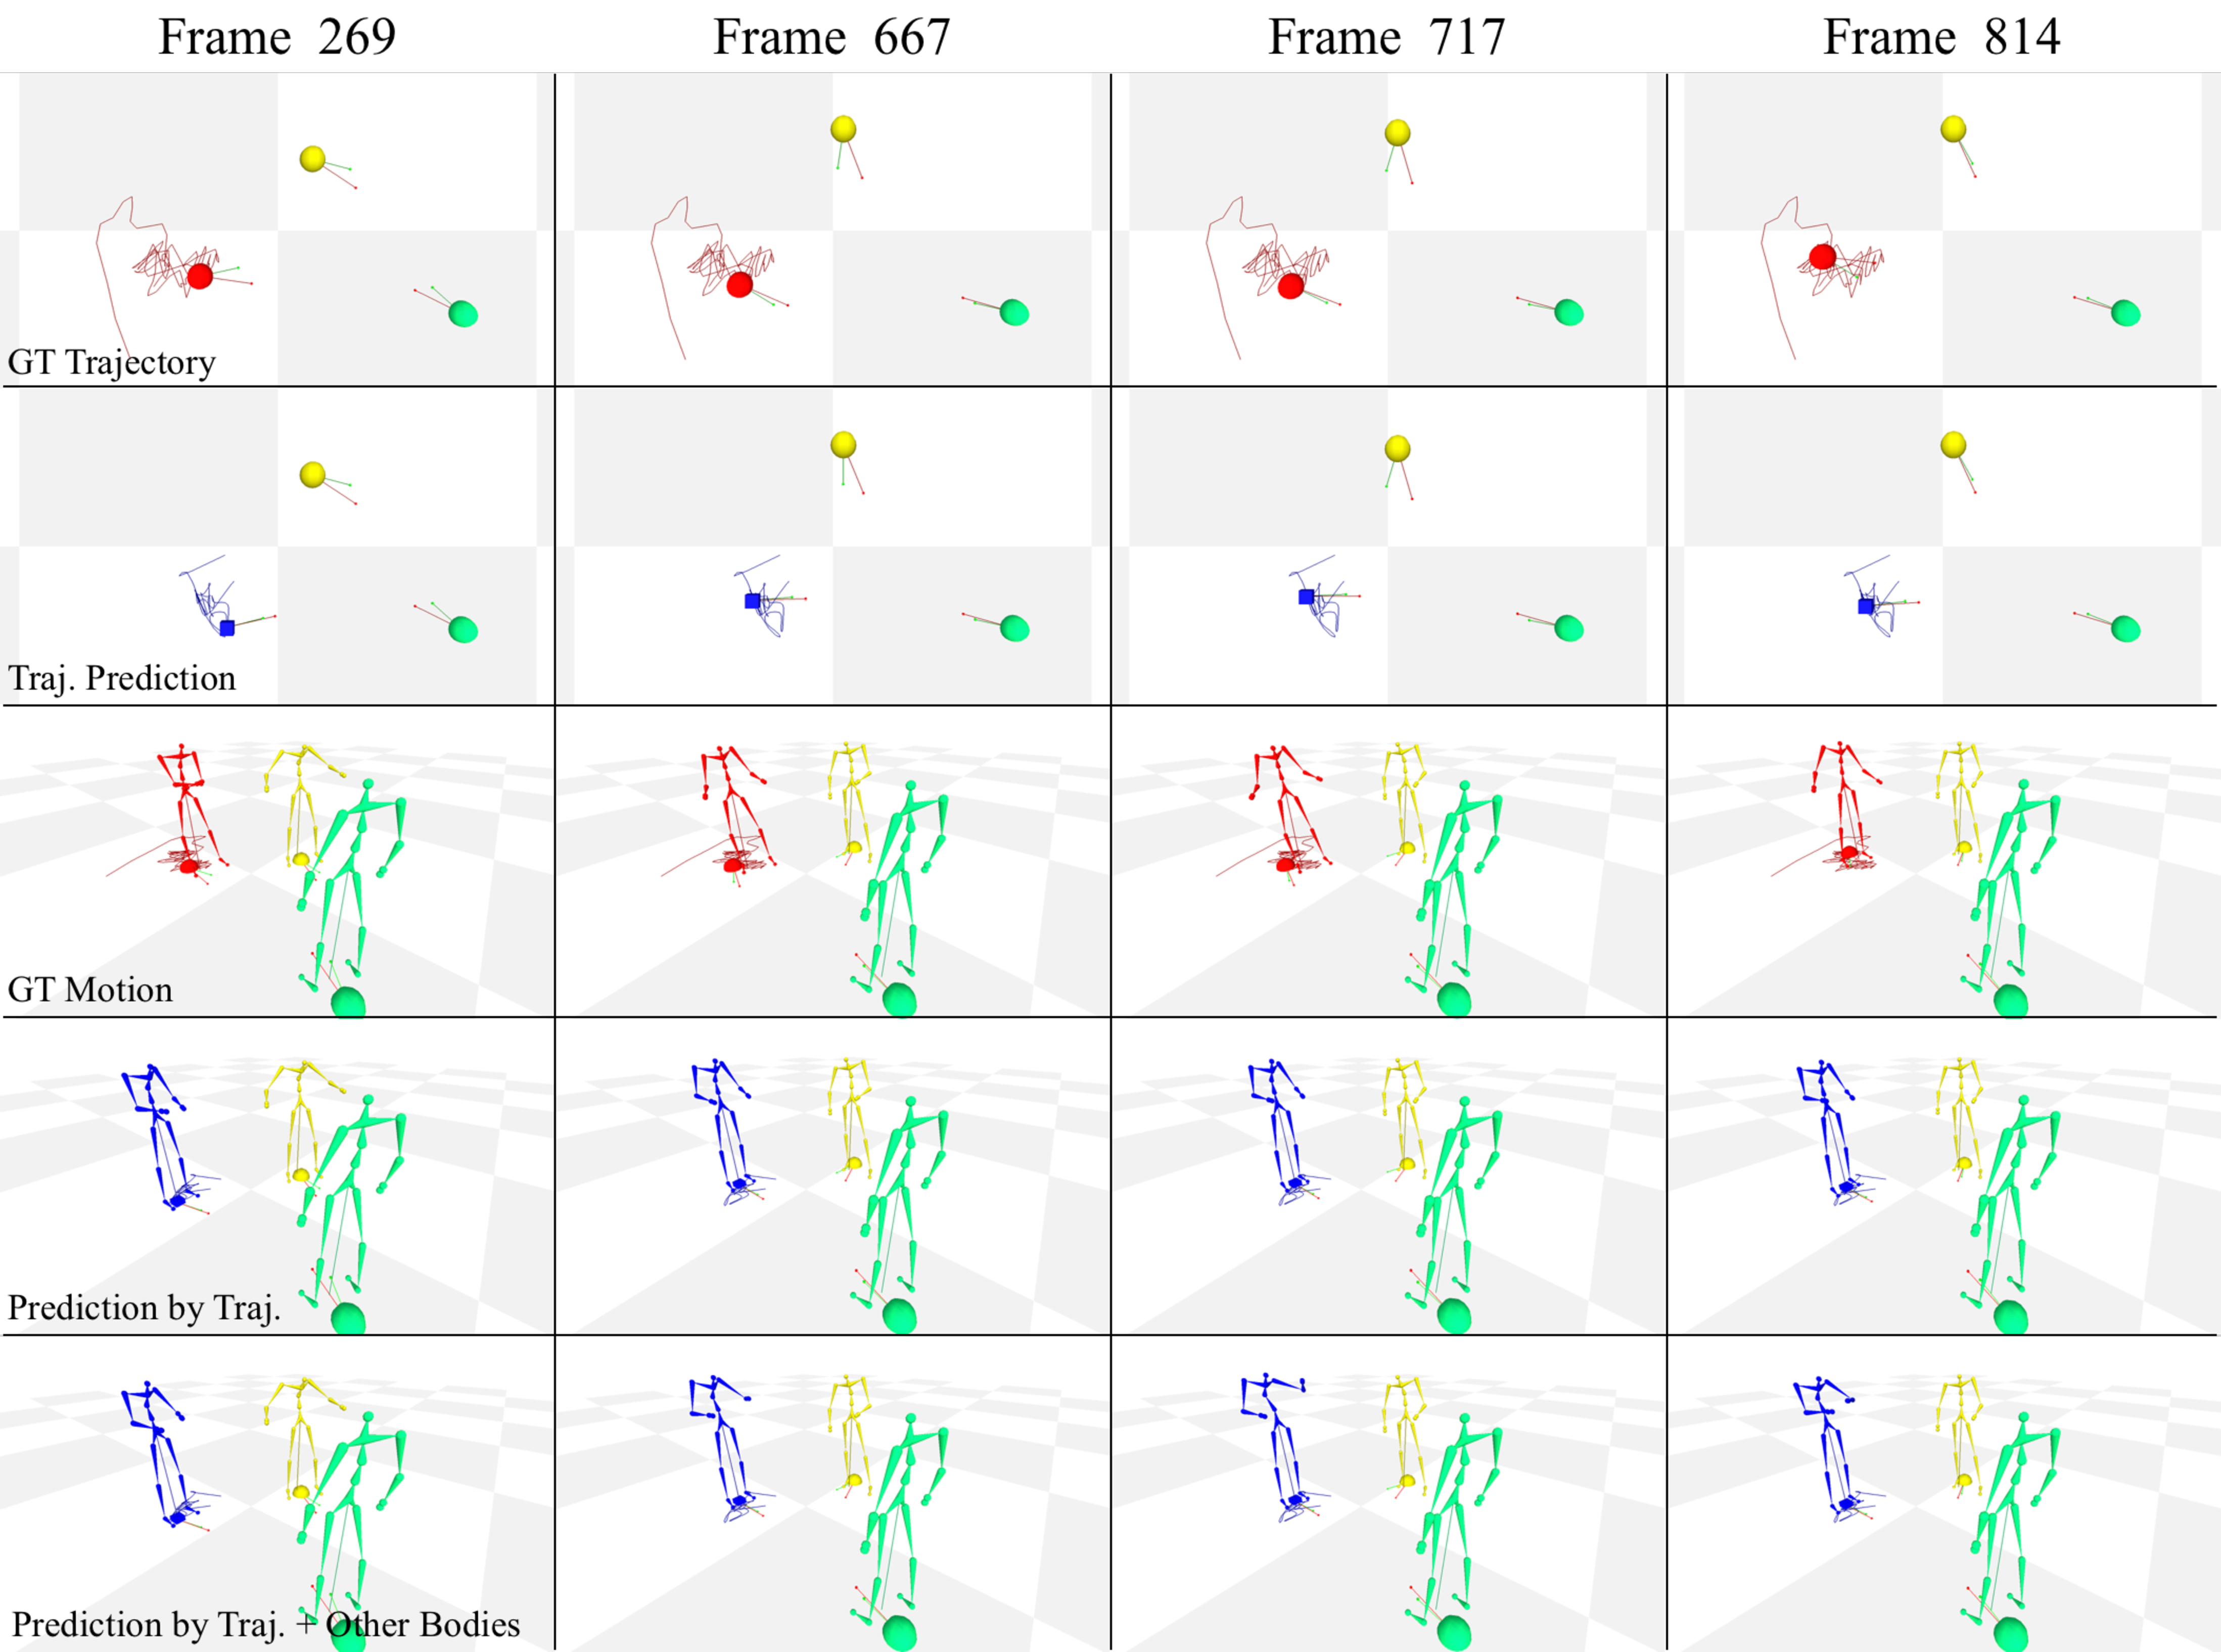
\includegraphics[width=\linewidth]{ssp_fig/qual_170221_b2_group4}
	%	\subfigure[TrajCompares]{\label{Fig:asso_traj}\includegraphics[width=0.5\textwidth]{img/trajCompare}}   
	\caption{An example result of \textit{Social Signal Prediction}. Each column shows scenes at a particular frame. The social signals drawn in green or yellow color are used as the inputs to our method, and blue signals are our social signal prediction results. The signals drawn in red are the ground truth. (First row) The ground truth social formations are shown from a top view, where the target person is shown as red spheres along with trajectories (red curves), face orientation (green arrows pointing from the spheres), and body orientations (red arrows from the spheres). (Second Row) The predicted locations (blue cubes), trajectories (blue curves), face orientations (green arrows), and body orientations (red arrows) are shown. (Third row) The ground-truth 3D body poses of the target person are shown. (Fourth row) We predict the 3D motion from the estimated 2D trajectory of the target person. (Fifth row) We use the body motion of other subjects to predict the upper body motion of the target person, which are combined to the leg body motions estimated from the trajectories.} 
	\label{fig:qualitative}
\end{figure*}

\begin{table}[t]
	\centering
	\footnotesize
	%\caption{Social Body Gesture Prediction Errors}
	\label{table:predBody_errors}
	\begin{tabular}{c| c| c}
		
		\hline
		%Types & Avg. dist. (cm) & Std.(cm) & Min dist. (cm)  & Max dist. (cm)\\
		Types & Avg. Joint Errors (cm) & Std.\\
		\hline
		%Mirroring buyer & 11.60 &2.70\\
		%\hline
		Mirroring input seller & 10.86 &2.49\\
		\hline
		Average body & \underline {\textbf{7.83}} & 2.33\\
		\hline
		Traj2Body & 8.31 & 2.26\\
		\hline
		% 		body2Body & 8.19 (2.01)\\
		Body2Body & 8.72 & 2.00\\
		\hline
		% 		body2Body & 8.19 (2.01)\\
		Hybrid & 8.61  & 1.84\\
		\hline
	\end{tabular}
	\caption{Social Body Gesture Prediction Errors (cm). Body orientation and face orientation are computed between estimated and GT unit vectors (need to be fixed)}
\end{table}



\subsection{Body Gestures Prediction}

We compute body motion of the target person by two methods. In the first method, the body motion is directly regressed from the estimated social formation (location and orientation) of the target person. This method shows leg motions following the trajectory movements, but has minimum upper body motion. Examples are shown in the fourth row of Fig.~\ref{fig:qualitative}. As an alternative method, we predict the target person's body motion by using other subjects' body motion as input. This motion does not take into account the global formation information, but shows more dynamic and realistic body motions by responding to other subjects' motion. Finally, we combine both methods, by merging the formation and leg motion from the first method to the upper body motion from the second method. Examples are shown in the fifth row of Fig.~\ref{fig:qualitative}. The final outputs predict more natural social behaviors than other baselines, satisfying most of the noticeable social rules in the scenes (distance, orientation, leg and root movement, and natural hand motions). Our results are best seen in the supplementary videos. However, the quantitative errors tend to be higher, as shown in Table~\ref{table:predBody_errors}. Notably, the average pose computed from the training set shows the best performance. This is because the error metric computing the 3D errors from the ground-truth cannot fully evaluate how natural the motion appears. %Given the similar social signal inputs, there are diverse possible suitable human motions, and a better evaluation method is required to consider this.%  the quality of social signal prediction.% and it should be related to a 

% {\color{red} Qualitative example where turn taking is captured?}

% \noindent \textbf{Direct Regression from Social Formations:}
% We can directly regress from the predicted 2D formation output.  

% PCK curves 
% Per joint


% \textbf{Regression from Richer Input:}
% We use other skeletons and input and see any improvement. 

% Compared to the direct regression. 
% {\color{red} Any semantic improvement which is not captured by numbers?}

% Any good way to evaluate realistic human motion???


% \subsection{Quantifying Social Signal Importance}



% \subsection{Correlation between Body, Face, and Hands}

% We use all body parts for communication where each part plays a role to send some specific signals. Unfortunately, these roles are also poorly understood. In this section, we investigate whether there exists patterns or strong correlations among parts. We study this by predicting a missing part given other body parts. 

% Body2face, face2body

% \subsection{Face and Hands signals}